\subsection{Coverage and source structure}

The retained index resolves 886 uploads to 180 nonempty publisher groups, with 39 uploads unresolved. The largest ten publishers contribute 38.0\% of attributed uploads and the largest twenty 66.9\%. This concentration describes index composition rather than audience size or practitioner prevalence.

The Q\&A layer contains 949 candidates from 67 of 75 digests. It spans 27 resolved publisher IDs, while 105 candidates remain in 7 unresolved inherited-name groups. All belong to one practitioner context. There are no literal transcript turns or verified answer-speaker labels in this candidate layer.

The conservative benchmark guard links uploads through exact normalized questions, question cosine at least 0.80, or at least three question-pair links at 0.40. It produces 55 groups from 67 Q\&A-bearing uploads, with 14 upload links, 8 multi-upload groups and a largest group of 4 uploads. The groups quarantine possible shared source material; they are not verified original-session identities.

\begin{figure*}[t]
\centering
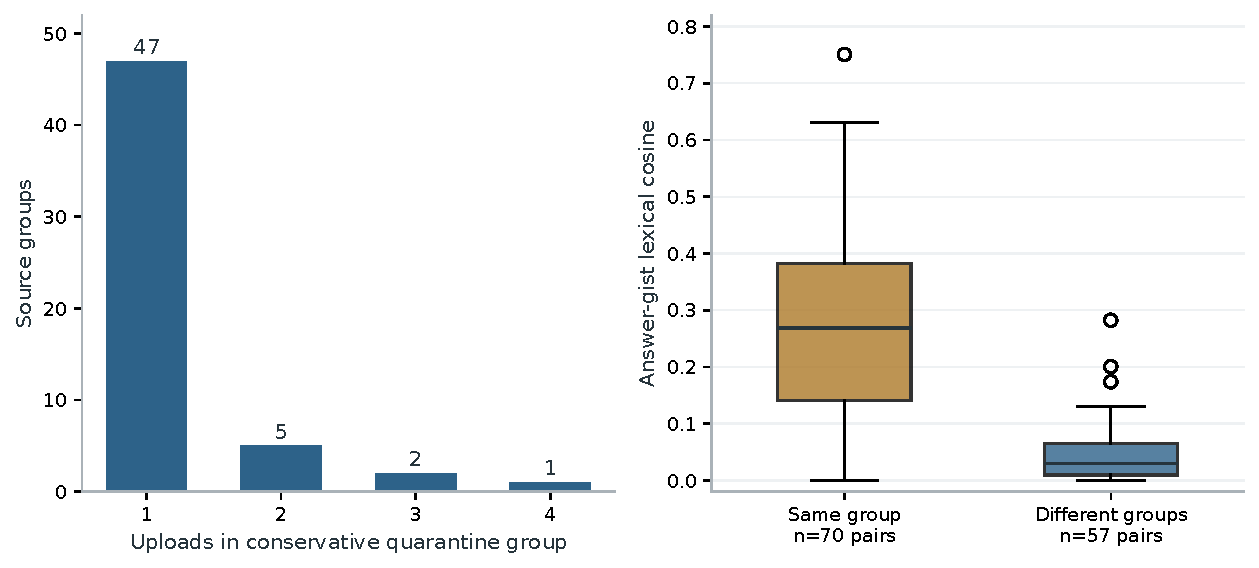
\includegraphics[width=\textwidth]{generated/figures/source-leakage-guard.pdf}
\caption{The conservative source guard changes which question neighbors are compared. Upload links are lexical dependency proxies. Same-group and cross-group pair distributions reuse candidates and are not independent samples or agreement scores.}
\label{fig:source-leakage-guard}
\end{figure*}

\subsection{Question similarity weakly predicts answer wording}

Across 441,797 distinct-upload candidate combinations, question and answer-gist lexical cosines have Spearman rank correlation 0.075. Aggregating to upload-pair means changes the association to 0.323. The change shows sensitivity to weighting and dependence, not a new independent sample.

The 127 question neighbors at cutoff 0.40 have mean answer-gist cosine 0.171. Restricting them to different quarantine groups leaves 57 pairs with mean 0.044. The 15 pairs with identical normalized question wording still have mean answer-gist cosine 0.311. None of these scores codes whether answers agree. Quarantine groups are themselves defined by exact/high question similarity or multiple retrieval links; this selected-pool change cannot isolate a source-reuse effect.

A second, explicitly exploratory comparison standardizes the within- and cross-quarantine answer means over question-cosine bins that contain both strata. The common-support pool contains 93 pairs (36 within and 57 cross), excluding 34 within-group pairs in high-similarity bins with no cross-group support. Pooled-bin weights applied identically to both strata give mean answer cosine 0.297 versus 0.044, a difference of 0.253. The directional within-group advantage is not disconfirmed by this sensitivity, but coarse bins leave prompt, length, topic and source-selection differences unresolved.

\begin{table*}[t]
\centering\small\setlength{\tabcolsep}{3pt}
\begin{tabular}{p{0.2\textwidth}p{0.12\textwidth}p{0.12\textwidth}p{0.17\textwidth}p{0.17\textwidth}p{0.12\textwidth}}
\toprule
Question-cosine band & Within pairs & Cross pairs & Within answer mean & Cross answer mean & Weight \\ \midrule
0.40--<0.50 & 16 & 38 & 0.356 & 0.039 & 0.581 \\
0.50--<0.60 & 14 & 12 & 0.203 & 0.026 & 0.280 \\
0.60--<0.70 & 6 & 7 & 0.243 & 0.104 & 0.140 \\
0.70--<0.80 & 10 & 0 & 0.229 & unavailable & excluded \\
0.80--<0.90 & 6 & 0 & 0.310 & unavailable & excluded \\
0.90--1.00 & 18 & 0 & 0.280 & unavailable & excluded \\
\bottomrule
\end{tabular}
\caption{Question-similarity common support. Standardization uses identical pooled-bin weights only where both quarantine strata occur. Missing cross-stratum means are not zero. These dependent-pair summaries are neither agreement scores nor causal estimates.}
\end{table*}

\begin{figure*}[t]
\centering
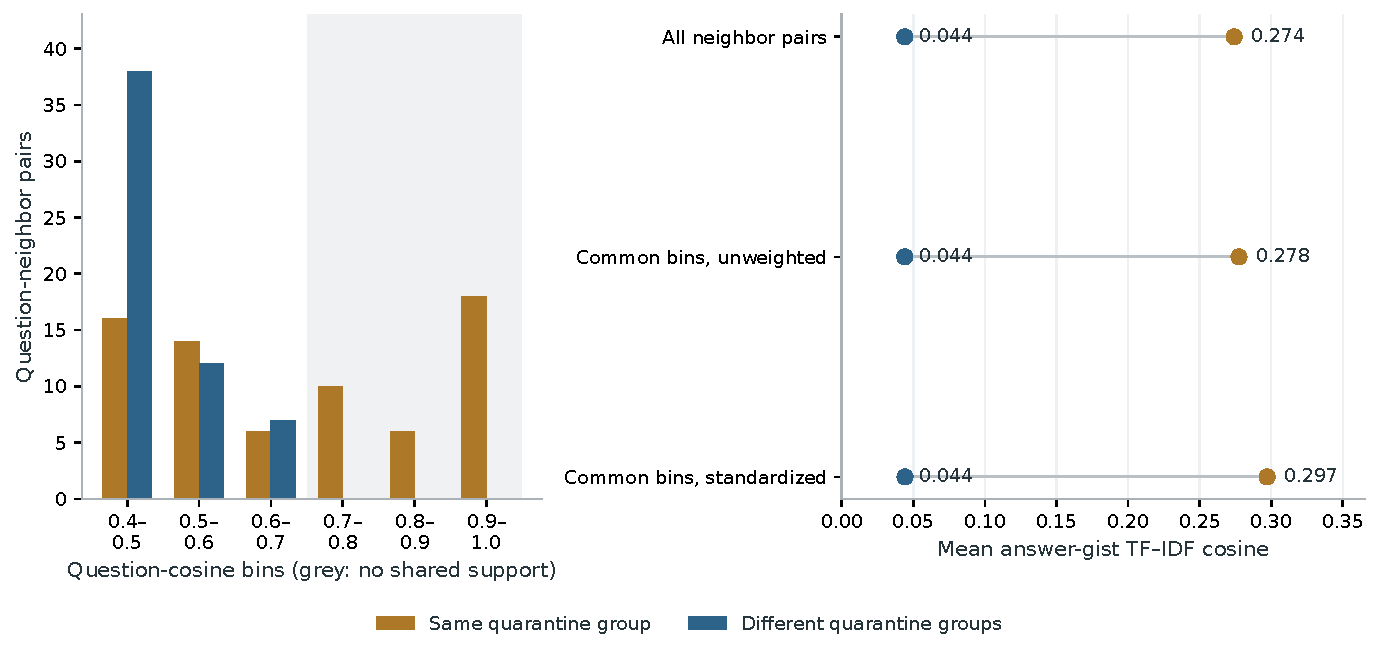
\includegraphics[width=\textwidth]{generated/figures/question-cosine-common-support.pdf}
\caption{Question-similarity support and standardized answer-gist contrast. Only three bins contain both strata: 93 retained pairs and 34 excluded higher-similarity within-group pairs. Identical pooled-bin weights yield descriptive means, with null unsupported comparisons. Group construction and remaining within-bin differences prevent a causal reuse or agreement interpretation.}
\label{fig:question-cosine-common-support}
\end{figure*}

\begin{figure*}[t]
\centering
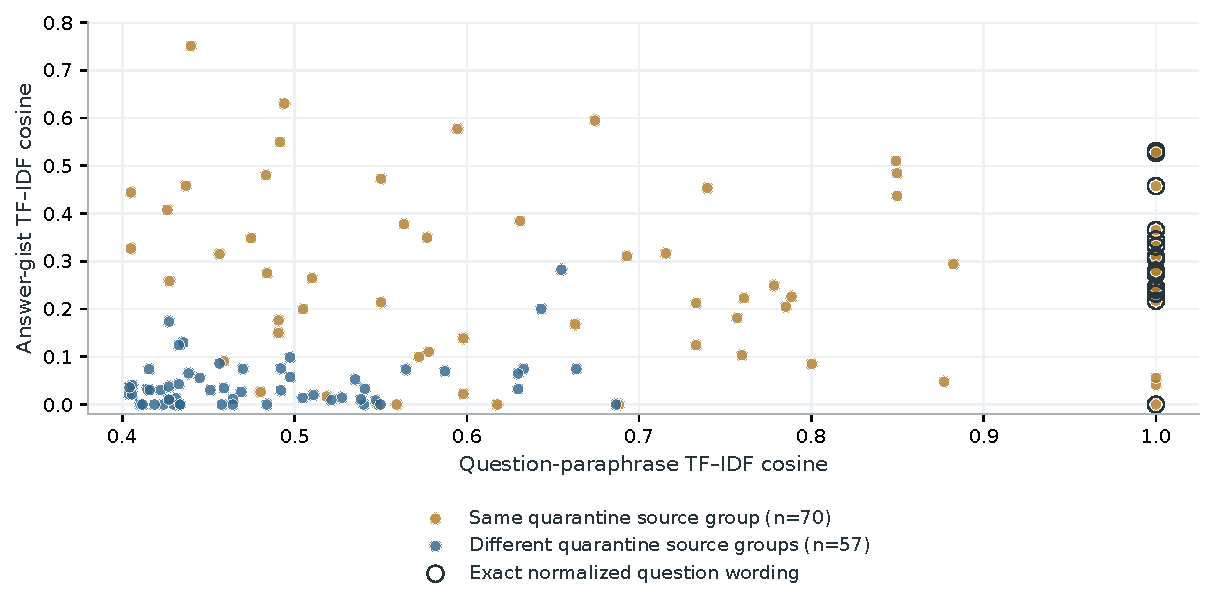
\includegraphics[width=\textwidth]{generated/figures/question-answer-alignment.pdf}
\caption{Question and answer-gist lexical resemblance on source-addressable candidate pairs. Question and answer TF--IDF fits are separate. The quarantine contrast is a dependency sensitivity, not a causal source effect or a semantic agreement validation.}
\label{fig:question-answer-alignment}
\end{figure*}

\subsection{Lexical neighborhoods change with their retrieval threshold}

At question cutoff 0.40, 178 of 949 candidates participate in nonsingleton lexical components; the largest contains 15 candidates. Raising the cutoff to 0.90 leaves 30 linked candidates and a largest component of 3. These are graph neighborhoods under a word-based rule, not validated topic clusters.

\begin{table}[t]
\centering\small\setlength{\tabcolsep}{3pt}
\begin{tabular}{p{0.2\columnwidth}p{0.15\columnwidth}p{0.23\columnwidth}p{0.29\columnwidth}}
\toprule
Cosine cutoff & Edges & Linked Qs & Largest component \\ \midrule
0.40 & 127 & 178 & 15 \\
0.50 & 73 & 114 & 10 \\
0.60 & 47 & 78 & 4 \\
0.70 & 34 & 58 & 3 \\
0.80 & 24 & 39 & 3 \\
0.90 & 18 & 30 & 3 \\
\bottomrule
\end{tabular}
\caption{Lexical graph sensitivity. Isolated candidates remain part of the 949-row denominator; graph connectivity is not original-session identity.}
\end{table}

\begin{figure*}[t]
\centering
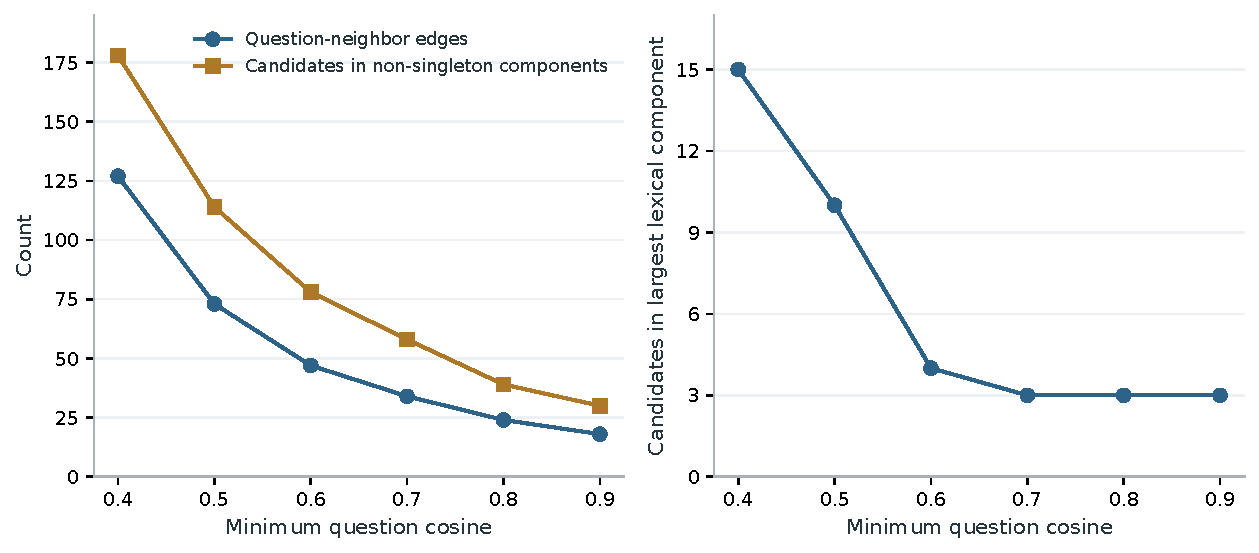
\includegraphics[width=\textwidth]{generated/figures/lexical-graph-stability.pdf}
\caption{Lexical-neighbor connectivity as the question cosine cutoff changes. Vertices are digest candidates and edges link different uploads. Component size reflects the chosen retrieval rule rather than a calibrated semantic or ontological category.}
\label{fig:lexical-graph-stability}
\end{figure*}

\subsection{Text-layer association changes after length conditioning}

The matched representation analysis uses 25 uploads from 14 publishers, yielding 300 dependent upload pairs (11 within publisher, 289 between). Raw title/caption cosine rank association is 0.249. After separate rank projections on absolute log duration ratio, mean log duration and absolute log caption-word ratio, the residual association is 0.129. Publisher omission yields -0.026--0.207, an influence range rather than a confidence interval.

Caption within-minus-between separation changes from 0.154 to 0.133 under the documented conditioning, while title separation changes from 0.229 to 0.217. These descriptive residual comparisons do not identify causal mediation or remove speaker and editing differences.

\begin{figure*}[t]
\centering
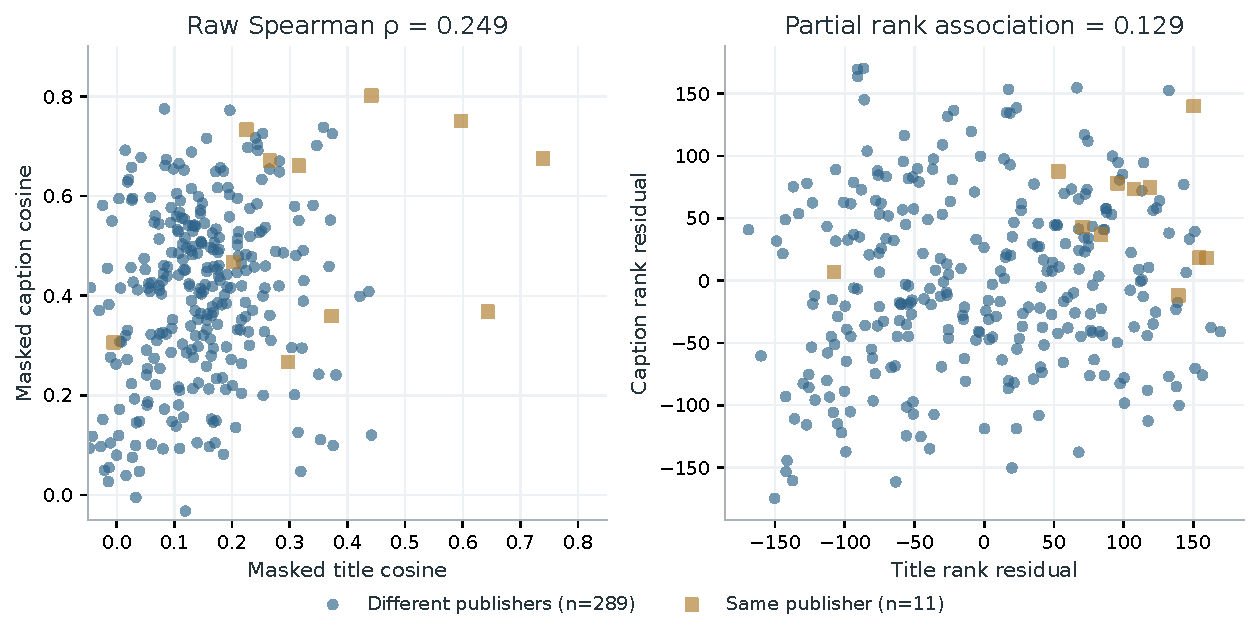
\includegraphics[width=\textwidth]{generated/figures/caption-duration-controls.pdf}
\caption{Title/caption association before and after measured length conditioning on identical uploads. Partial rank association is the correlation of separately projected rank residuals. Pair entries share uploads; publisher-omission ranges measure influence.}
\label{fig:caption-duration-controls}
\end{figure*}

\subsection{Local generation and adaptation pilot}

The executed pilot uses \texttt{Qwen/Qwen2.5-0.5B-Instruct}, revision \texttt{7ae557604adf} (full revision in the run receipt), under its Apache-2.0 license. It uses 48 training examples from 47 source-proxy groups and 8 questions from 8 disjoint groups, plus 2 unsupported-input controls. The retrieval store contains only the training examples; held-out answers are deliberately absent. This is a sparse-source transfer stress test, not a conventional factual RAG benchmark with known answer-bearing documents.

\begin{table*}[t]
\centering\small\setlength{\tabcolsep}{3pt}
\begin{tabular}{p{0.34\textwidth}p{0.15\textwidth}p{0.22\textwidth}p{0.2\textwidth}}
\toprule
Arm & Token F1 & Seconds / response & Strict control marker \\ \midrule
Lexical retrieval & 0.035 & 0.0004 & 1/2 \\
Base closed-book & 0.060 & 1.3962 & 0/2 \\
Base + retrieval & 0.011 & 1.3260 & 1/2 \\
LoRA closed-book & 0.145 & 3.2899 & 0/2 \\
LoRA + retrieval & 0.012 & 1.7715 & 2/2 \\
\bottomrule
\end{tabular}
\caption{Eight held-out question gists and two controls per arm. F1 is lexical overlap with an AI-produced reference gist. Control column counts exact INSUFFICIENT\_EVIDENCE marker emission, not all semantic refusal. The extractive baseline copies a full gist; generators are capped at 40 new tokens. Latency excludes model loading and index fitting. No model-quality ranking is inferred.}
\end{table*}

LoRA executes 48 microsteps and 12 optimizer updates over one epoch in 65.04 seconds, adapting 270,336 of 494,303,104 parameters. Rank is 4 with alpha 8, learning rate 0.0002, gradient accumulation 4, and targets \texttt{q\_proj} and \texttt{v\_proj}. Peak process RSS is 3.21 GiB. This is a short adaptation smoke test on a shared CPU, not an optimized training study or CPU/GPU comparison.

Closed-book reference overlap changes from 0.060 to 0.145 after adaptation, while retrieval-conditioned values are 0.011 and 0.012. The missing held-out answers in the retrieval store confound any algorithm ranking: low overlap may accompany appropriate refusal or evidence gaps. Both language-model retrieval arms emit no valid evidence-label citation on the held-out questions. Citation compliance is therefore an observed failure, separate from source entailment.

The strict control score counts a literal marker. A base response saying ``Insufficient evidence. is a semantic refusal but does not match that marker; zero strict score must not be described as zero refusal. Conversely, the adapted closed-book output supplies a studio temperature of 23 degrees Celsius although no measurement evidence is provided. This concrete unsupported assertion is a substantive failure that token F1 cannot diagnose. The controls are diagnostic examples, not a representative hallucination rate.

A separately disclosed post-hoc phrase diagnostic was defined after inspecting the responses; it does not replace the original metric. It matches refusal expressions such as ``insufficient evidence with spaces/underscores and ``not available. It is another lexical rule, not a human semantic-refusal annotation.

\begin{table}[t]
\centering\small\setlength{\tabcolsep}{3pt}
\begin{tabular}{p{0.43\columnwidth}p{0.24\columnwidth}p{0.24\columnwidth}}
\toprule
Arm & Strict marker & Post-hoc phrase hits \\ \midrule
Lexical retrieval & 1/2 & 1/2 \\
Base closed-book & 0/2 & 2/2 \\
Base + retrieval & 1/2 & 2/2 \\
LoRA closed-book & 0/2 & 1/2 \\
LoRA + retrieval & 2/2 & 2/2 \\
\bottomrule
\end{tabular}
\caption{Control diagnostics on the same two unsupported inputs per arm. The post-hoc phrase rule was selected after viewing outputs and is not an independent validation set.}
\end{table}

Four additional answer-present positive controls supply an exact training-source question and gist, separately for base and adapted retrieval. They are not held-out tests and are excluded from the original five-arm table. Of 4 outputs, 2 exactly reproduce the supplied gist under token-overlap F1, yet 0 emit a valid evidence-label citation. Source availability therefore does not repair citation compliance in this diagnostic. Reproducing an attributed source assertion remains distinct from externally verifying it.

Generation is greedy, float32, limited to 40 new tokens and a 512-token prompt. No prompt was truncated; 5 adapted closed-book and 1 adapted retrieval responses hit the generation cap. Length-limited outputs can lose qualifications and depress lexical overlap. Their full outputs and source evidence remain inspectable in the prediction archive.


\begin{figure*}[t]
\centering
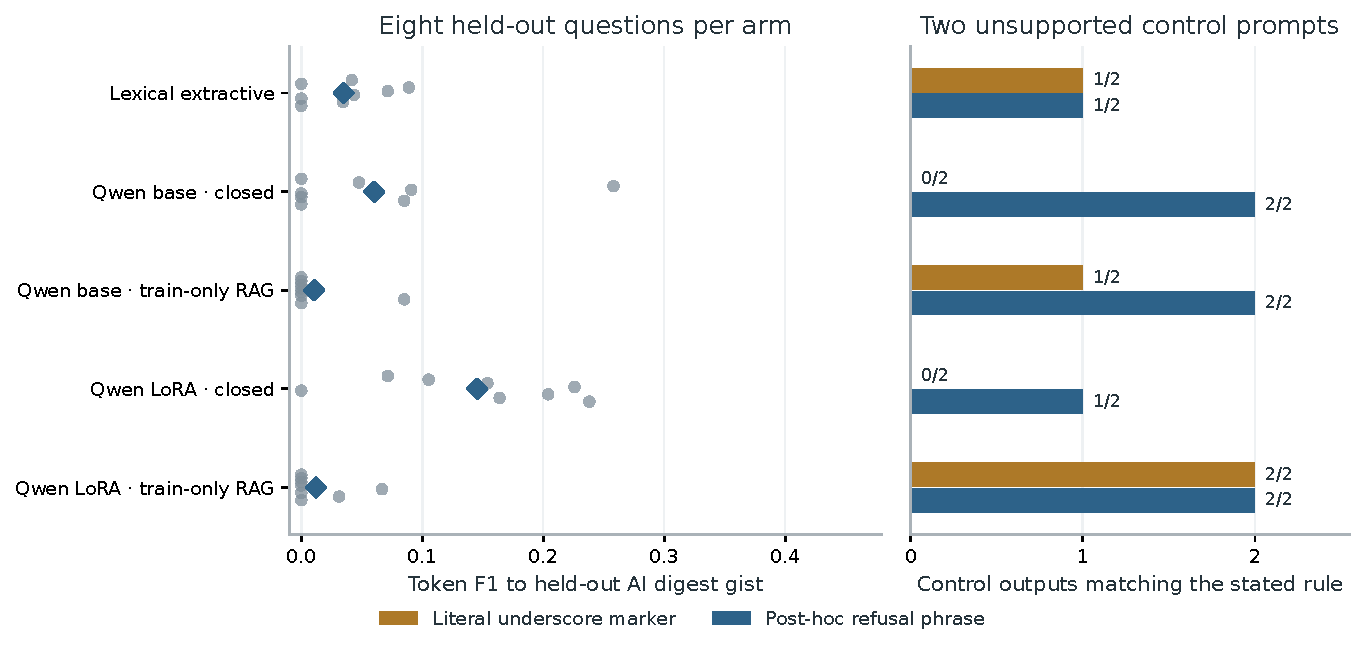
\includegraphics[width=\textwidth]{generated/figures/model-reconstruction-controls.pdf}
\caption{Five executed pilot arms: held-out lexical gist overlap, strict control-marker emission (gold) and the separately defined post-hoc refusal-phrase rule (blue). Eight references are AI digest gists; two controls test unsupported inputs. Neither control rule is human refusal accuracy. Train-only retrieval excludes held-out answers, so these quantities do not rank factual model quality.}
\label{fig:model-reconstruction-controls}
\end{figure*}

\subsection{Structured content labeling exposes another failure mode}

An additional base-model task inspects 12 digest excerpts from distinct source-proxy groups, balanced by a dictionary conditionality marker. It requests a primary answer-orientation label, a conditionality label and an exact evidence span of at most eight words. Only 9 outputs parse under the requested schema; 3 remain recorded failures. Conditional labels match the dictionary method in 5/9 parseable cases. This is method concordance on a selected set, not human annotation accuracy.

The most frequent parsed primary label is contact\_forecast (9/9 parseable outputs). Conditional wording is labeled yes in 9/9 parseable cases, so the reported dictionary concordance is compatible with a collapsed single-label response. Only 0 of 9 parseable evidence spans satisfy the exact-short-span rule. Forced single labels and overlapping dictionary categories are not equivalent tasks. These failures argue for retaining raw outputs and explicit unknown/parse states before using generated labels to characterize this material; they do not establish corpus-wide topic prevalence.

A final same-item probe changes only the listed theme-option order, keeping the twelve excerpts, conditional options and generation settings fixed. Original and reversed prompts each yield 9 parseable outputs, with 8 items parseable in both conditions. Of those paired items, 6 change primary theme. The reversed list yields 7 personal-practice and 2 contact/forecast labels, but selects the new first option in 0/9 parseable outputs. This disconfirms a simple first-option-copying explanation while demonstrating local prompt-order sensitivity. No reversed output satisfies the combined exact-short-span rule.

A separate post-hoc dictionary sensitivity narrows the broad dependency-word expression. Conditional flags change from 60 to 58 among 949 source gists (2 changed records). Neither rule is a human reference, and the original selection and benchmark labels remain unchanged. Stability under this single lexical perturbation does not validate the conditionality construct.

The newer pinned Qwen3.5-0.8B model then executes the same twelve excerpts and original annotation schema/options with a 96-token cap, greedy decoding and thinking disabled. It returns 12/12 parseable outputs and 5/12 exact answer substrings of at most eight words, compared with 9/12 and 0/9 in the original small-model run. Its conditional labels are yes in 12/12 cases: 6/12 dictionary concordance is exactly the always-yes result on the balanced six/six sample. Primary labels remain concentrated (11 personal-practice, 1 contact/forecast).

Thus parsing and short-span compliance improve in this same-item check while conditional-label collapse persists. Of the newer model's 12 evidence strings, 10 are exact contiguous answer substrings; 5 of those exceed eight words, leaving 5 combined exact-short successes and 2 nonexact strings. Exact but overlength spans are length-compliance failures, not invented evidence. The modern model uses its own tokenizer/chat template and runtime; architecture, instruction behavior and those implementation changes are not isolated. Mean runtime is 6.90 seconds per excerpt, with 0 cap hits and peak process RSS 5.35 GiB. No human label accuracy, source-truth validation or general model ranking is established.

\begin{table*}[t]
\centering\small\setlength{\tabcolsep}{3pt}
\begin{tabular}{p{0.25\textwidth}p{0.16\textwidth}p{0.18\textwidth}p{0.18\textwidth}p{0.16\textwidth}}
\toprule
Annotation condition & Parsed / selected & Exact spans / parsed & Exact + short / parsed & Primary labels \\ \midrule
Qwen2.5 original & 9/12 & 0/9 & 0/9 & 9 contact/forecast \\
Qwen2.5 reversed options & 9/12 & 0/9 & 0/9 & 7 personal practice; 2 contact/forecast \\
Qwen3.5 original options & 12/12 & 10/12 & 5/12 & 11 personal practice; 1 contact/forecast \\
\bottomrule
\end{tabular}
\caption{Same selected excerpts, explicitly different prompt/model conditions. Exact means a nonempty contiguous answer substring; the combined criterion also requires at most eight whitespace words. Source labels are model outputs, not measured corpus prevalence or human annotation accuracy.}
\end{table*}

\subsection{Newer-family execution is a separate compatibility probe}

A separately pinned \texttt{Qwen/Qwen3.5-0.8B} model, revision \texttt{2fc06364715b}, also executes on CPU using \texttt{Transformers 5.20.2}. The single text-only prompt directly supplies the desired provenance values (AI digest and unverified speaker turns) and requests a JSON object. The response follows that schema. This is instruction-following compatibility, not independently inferred provenance, domain accuracy or a comparison with the earlier labeling task.

The probe generates 23 tokens under a 32-token limit in 3.88 seconds after 1.03 seconds of model loading, with peak process RSS 5.33 GiB. The architecture supports image/text inputs, but no image, video, audio or speech-recognition input is used. Its different prompt and budget make it separate from the five-arm Qwen2.5 experiment; no state-of-the-art, model-quality or CPU/GPU ranking follows.
